\documentclass[12pt,a4paper]{article}
\usepackage{ctex}
\usepackage{amsmath,amscd,amsbsy,amssymb,latexsym,url,bm,amsthm}
\usepackage{epsfig,graphicx,subfigure}
\usepackage{enumitem,balance}
\usepackage{wrapfig}
\usepackage{mathrsfs,euscript}
\usepackage[usenames]{xcolor}
\usepackage{hyperref}
\usepackage[vlined,ruled,linesnumbered]{algorithm2e}
\usepackage{array}
\hypersetup{colorlinks=true,linkcolor=black}

\newtheorem{theorem}{Theorem}
\newtheorem{lemma}[theorem]{Lemma}
\newtheorem{proposition}[theorem]{Proposition}
\newtheorem{corollary}[theorem]{Corollary}
\newtheorem{exercise}{Exercise}
\newtheorem*{solution}{Solution}
\newtheorem{definition}{Definition}
\theoremstyle{definition}

\renewcommand{\thefootnote}{\fnsymbol{footnote}}

\newcommand{\postscript}[2]
 {\setlength{\epsfxsize}{#2\hsize}
  \centerline{\epsfbox{#1}}}

\renewcommand{\baselinestretch}{1.0}

\setlength{\oddsidemargin}{-0.365in}
\setlength{\evensidemargin}{-0.365in}
\setlength{\topmargin}{-0.3in}
\setlength{\headheight}{0in}
\setlength{\headsep}{0in}
\setlength{\textheight}{10.1in}
\setlength{\textwidth}{7in}
\makeatletter \renewenvironment{proof}[1][Proof] {\par\pushQED{\qed}\normalfont\topsep6\p@\@plus6\p@\relax\trivlist\item[\hskip\labelsep\bfseries#1\@addpunct{.}]\ignorespaces}{\popQED\endtrivlist\@endpefalse} \makeatother
\makeatletter
\renewenvironment{solution}[1][Solution] {\par\pushQED{\qed}\normalfont\topsep6\p@\@plus6\p@\relax\trivlist\item[\hskip\labelsep\bfseries#1\@addpunct{.}]\ignorespaces}{\popQED\endtrivlist\@endpefalse} \makeatother

\begin{document}
\noindent

%========================================================================
\noindent\framebox[\linewidth]{\shortstack[c]{
\Large{\textbf{Lab10-Turing Machine}}\vspace{1mm}\\
CS214-Algorithm and Complexity, Xiaofeng Gao \& Lei Wang, Spring 2021.}}
\begin{center}
\footnotesize{\color{red}$*$ If there is any problem, please contact TA Yihao Xie. }

\footnotesize{\color{blue}$*$ Name:Renyang Guanajuato  \quad Student ID:519021911058 \quad Email: guanrenyang@sjtu.edu.cn}
\end{center}

\begin{enumerate}
    \item Design a one-tape TM $M$ that computes the function $f(x, y) = \lfloor x/y \rfloor$, where $x$ and $y$ are positive integers $(x > y)$. The alphabet is $\{1, 0, \Box, \triangleright, \triangleleft\}$, and the inputs are $x$ "1"s, $\Box$ and $y$ "1"s. Below is the initial configuration for input $x=7$ and $y=3$. The result $z=f(x,y)$ should also be represented in the form of $z$ "1"s on the tape with pattern of $\rhd 111\cdots 111\lhd$, which is $\rhd 11\lhd$ for the example.
    
	\begin{center}
		\begin{tabular}{ll|c|c|c|c|c|c|c|c|c|c|c|c|c|c}
			& \multicolumn{14}{c}{Initial Configuration}\\[5pt]
			\cline{2-16}
			& & $\triangleright$ &  1  & 1 & 1 & 1 & 1 & 1 & 1 & $\Box$ & 1 & 1 & 1 & $ \triangleleft$ & \\
			\cline{2-16}
			\multicolumn{2}{c}{} & \multicolumn{1}{c}{$\uparrow$} & \multicolumn{11}{c}{}\\[-4pt]
			\multicolumn{2}{c}{} & \multicolumn{1}{c}{$q_S$} & \multicolumn{11}{c}{}	
		\end{tabular}
	\end{center}

    \begin{enumerate}
	\item
	Please describe your design and then write the specifications of $M$ in the form like $\langle q_S, \triangleright \rangle \rightarrow \langle q_1, \triangleright,  R\rangle$. Explain the transition functions in detail.
	
	\item
	Please draw the state transition diagram.
	
	\item
	Show briefly and clearly the whole process from initial to final configurations for input $x = 7$ and $y = 3$. You may start like this:
	$$(q_s,\underline{\triangleright}  1  1  1  1  1  1  1  \Box 1  1  1   \triangleleft)
	\vdash (q_1,\triangleright  \underline{1}  1  1  1  1  1  1  \Box 1  1  1   \triangleleft)
	\vdash^* (q_1,\triangleright  1  1  1  1  1  1  1  \underline{\Box} 1  1  1   \triangleleft)
	\vdash (q_2,\triangleright  1  1  1  1  1  1  1  \Box \underline{1}  1  1   \triangleleft)$$
	
	\par{\color{blue}(Note that for simplicity, we write $(q_1,\triangleright  \underline{1}  1  1  1  1  1  1  \Box 1  1  1   \triangleleft)\vdash^* (q_1,\triangleright  1  1  1  1  1  1  1  \underline{\Box} 1  1  1   \triangleleft)$ if the corresponding transaction repeats on multiple inputs with the same state.)}
	
\end{enumerate}
	
	\begin{solution}
	~\\
	\begin{enumerate}
	\item \textbf{\textit{Transition functions:}}
	\begin{center}
		$<q_s,1>\rightarrow <q_s,1,R>$ \quad $<q_s,\triangleright >\rightarrow <q_s,\triangleright ,R>$\\
		$<q_s,\Box >\rightarrow <q_1,\Box ,R>$\quad
		 $<q_1,1>\rightarrow <q_2,0,L>$\\ $<q_1,0>\rightarrow <q_1,0,R>$\quad
		 $<q_1,\Box >\rightarrow <q_1,\Box ,R>$\\ $<q_1,\triangleleft >\rightarrow <q_3,\triangleleft,R>$\quad $<q_2,1>\rightarrow <q_1,\Box ,R>$\\
		 $<q_2,0>\rightarrow <q_2,0,L>$\quad $<q_2,\triangleright >\rightarrow <q_5,\Box ,R>$\\
		 $<q_2,\Box >\rightarrow <q_2,\Box ,L>$\quad $<q_3,1>\rightarrow <q_3,1,R>$\\
		 $<q_3,\Box>\rightarrow <q_4,1,L>$\quad $<q_4,1>\rightarrow <q_4,1,L>$\\
		 $<q_4,0>\rightarrow <q_4,1,L>$\quad $<q_4,\Box>\rightarrow <q_1,\Box ,R>$\\
		 $<q_4,\triangleleft >\rightarrow <q_4,\triangleleft,L>$\quad
		 $<q_5,1>\rightarrow <q_5,\Box ,R>$\\ $<q_5,0>\rightarrow <q_5,\Box ,R>$\quad
		 $<q_5,\Box >\rightarrow <q_5,\Box ,R>$\\ $<q_5,\triangleleft>\rightarrow <q_6,\triangleright,R>$\quad
		 $<q_6,1>\rightarrow <q_6,1,R>$ \\ $<q_6,\Box>\rightarrow <q_{halt},\triangleleft,S>$
	\end{center}
	\textbf{\textit{Intuition of the algorithm:}}
	\\
	To compute $\lfloor x/y \rfloor$, we do $x\leftarrow x-y$ and add $1$ to the result circularly until $x<Y$. Since $x$ and $y$ are represented by $1$s, each time one bit of $y$ is read, the bit is set to $0$ to mark that this bit has been read. Then we set the corresponding bit of $x$ to $\Box$(setting one bit of $x$ to $\Box$ means $x$ is subtracted by $1$).
	\\
	\textbf{\textit{Explanation:}}
	\\
	\textbf{State $q_s$} scans the input sequence until the separator $\Box$ is found. As a result, the head moves right when it read $\triangleright$ or $1$.
	\\
	\textbf{State $q_1$} locates the first $1$ in the sequence of $y$ from the separator $\Box$, so the head moves right when it reads $0$ and $\Box$. When the head reads $1$, it sets the cell to $0$ and moves left to set one cell of $x$ to $\Box$ ($q_2$).
	\\
	\textbf{State $q_2$} will set the cell on the right side of $x$ to $\Box$ after the head reads $1$, so the head moves left when it reads $\Box$ and $0$. If the head reads $\triangleleft$ in state $q_2$, which means the left $1$s of $x$ is not enough to be divided by $y$, the head replaces $\triangleleft$ with $\Box$ go to state $q_5$.
	\\
	\textbf{State $q_3$} add $1$ to the result of the division after one $x\leftarrow x-y$, which is signed by reading $\triangleleft$ in state $q_1$. The result is stored after $\triangleleft$ so the head will move right when it reads $1$ and replaces the first $\Box$ it meet with $1$.
	\\
	\textbf{State $q_4$} resets $y$, currently being signed by $0$, to $1$. Consequently, the head moves left when it reads $1$ and $\triangleleft$, and replace $0$ with $1$ before move left. Then next $x\leftarrow x-y$ begins and the machine returns to state $q_1$ when the head reads $\Box$, which means the sequence of $y$ has been scanned. 
	\\
	\textbf{State $q_5$} replace the cells before the result with $\Box$ except for the cell next to the result, which is replaced by $\triangleright$. Consequently, the head replaces $1$ and $0$ with $\Box$ and $\triangleleft$ with $\triangleright$ before moving right. The machine goes into state $q_6$ after modifying $\triangleleft$.
	\\
	\textbf{State $q_6$} set the cell next to the end of the result sequence to $\triangleleft$ to ensure the format of the output.
	
	\item \textbf{\textit{Transition diagram:}}
	\begin{figure}[!htbp]
	\centering
	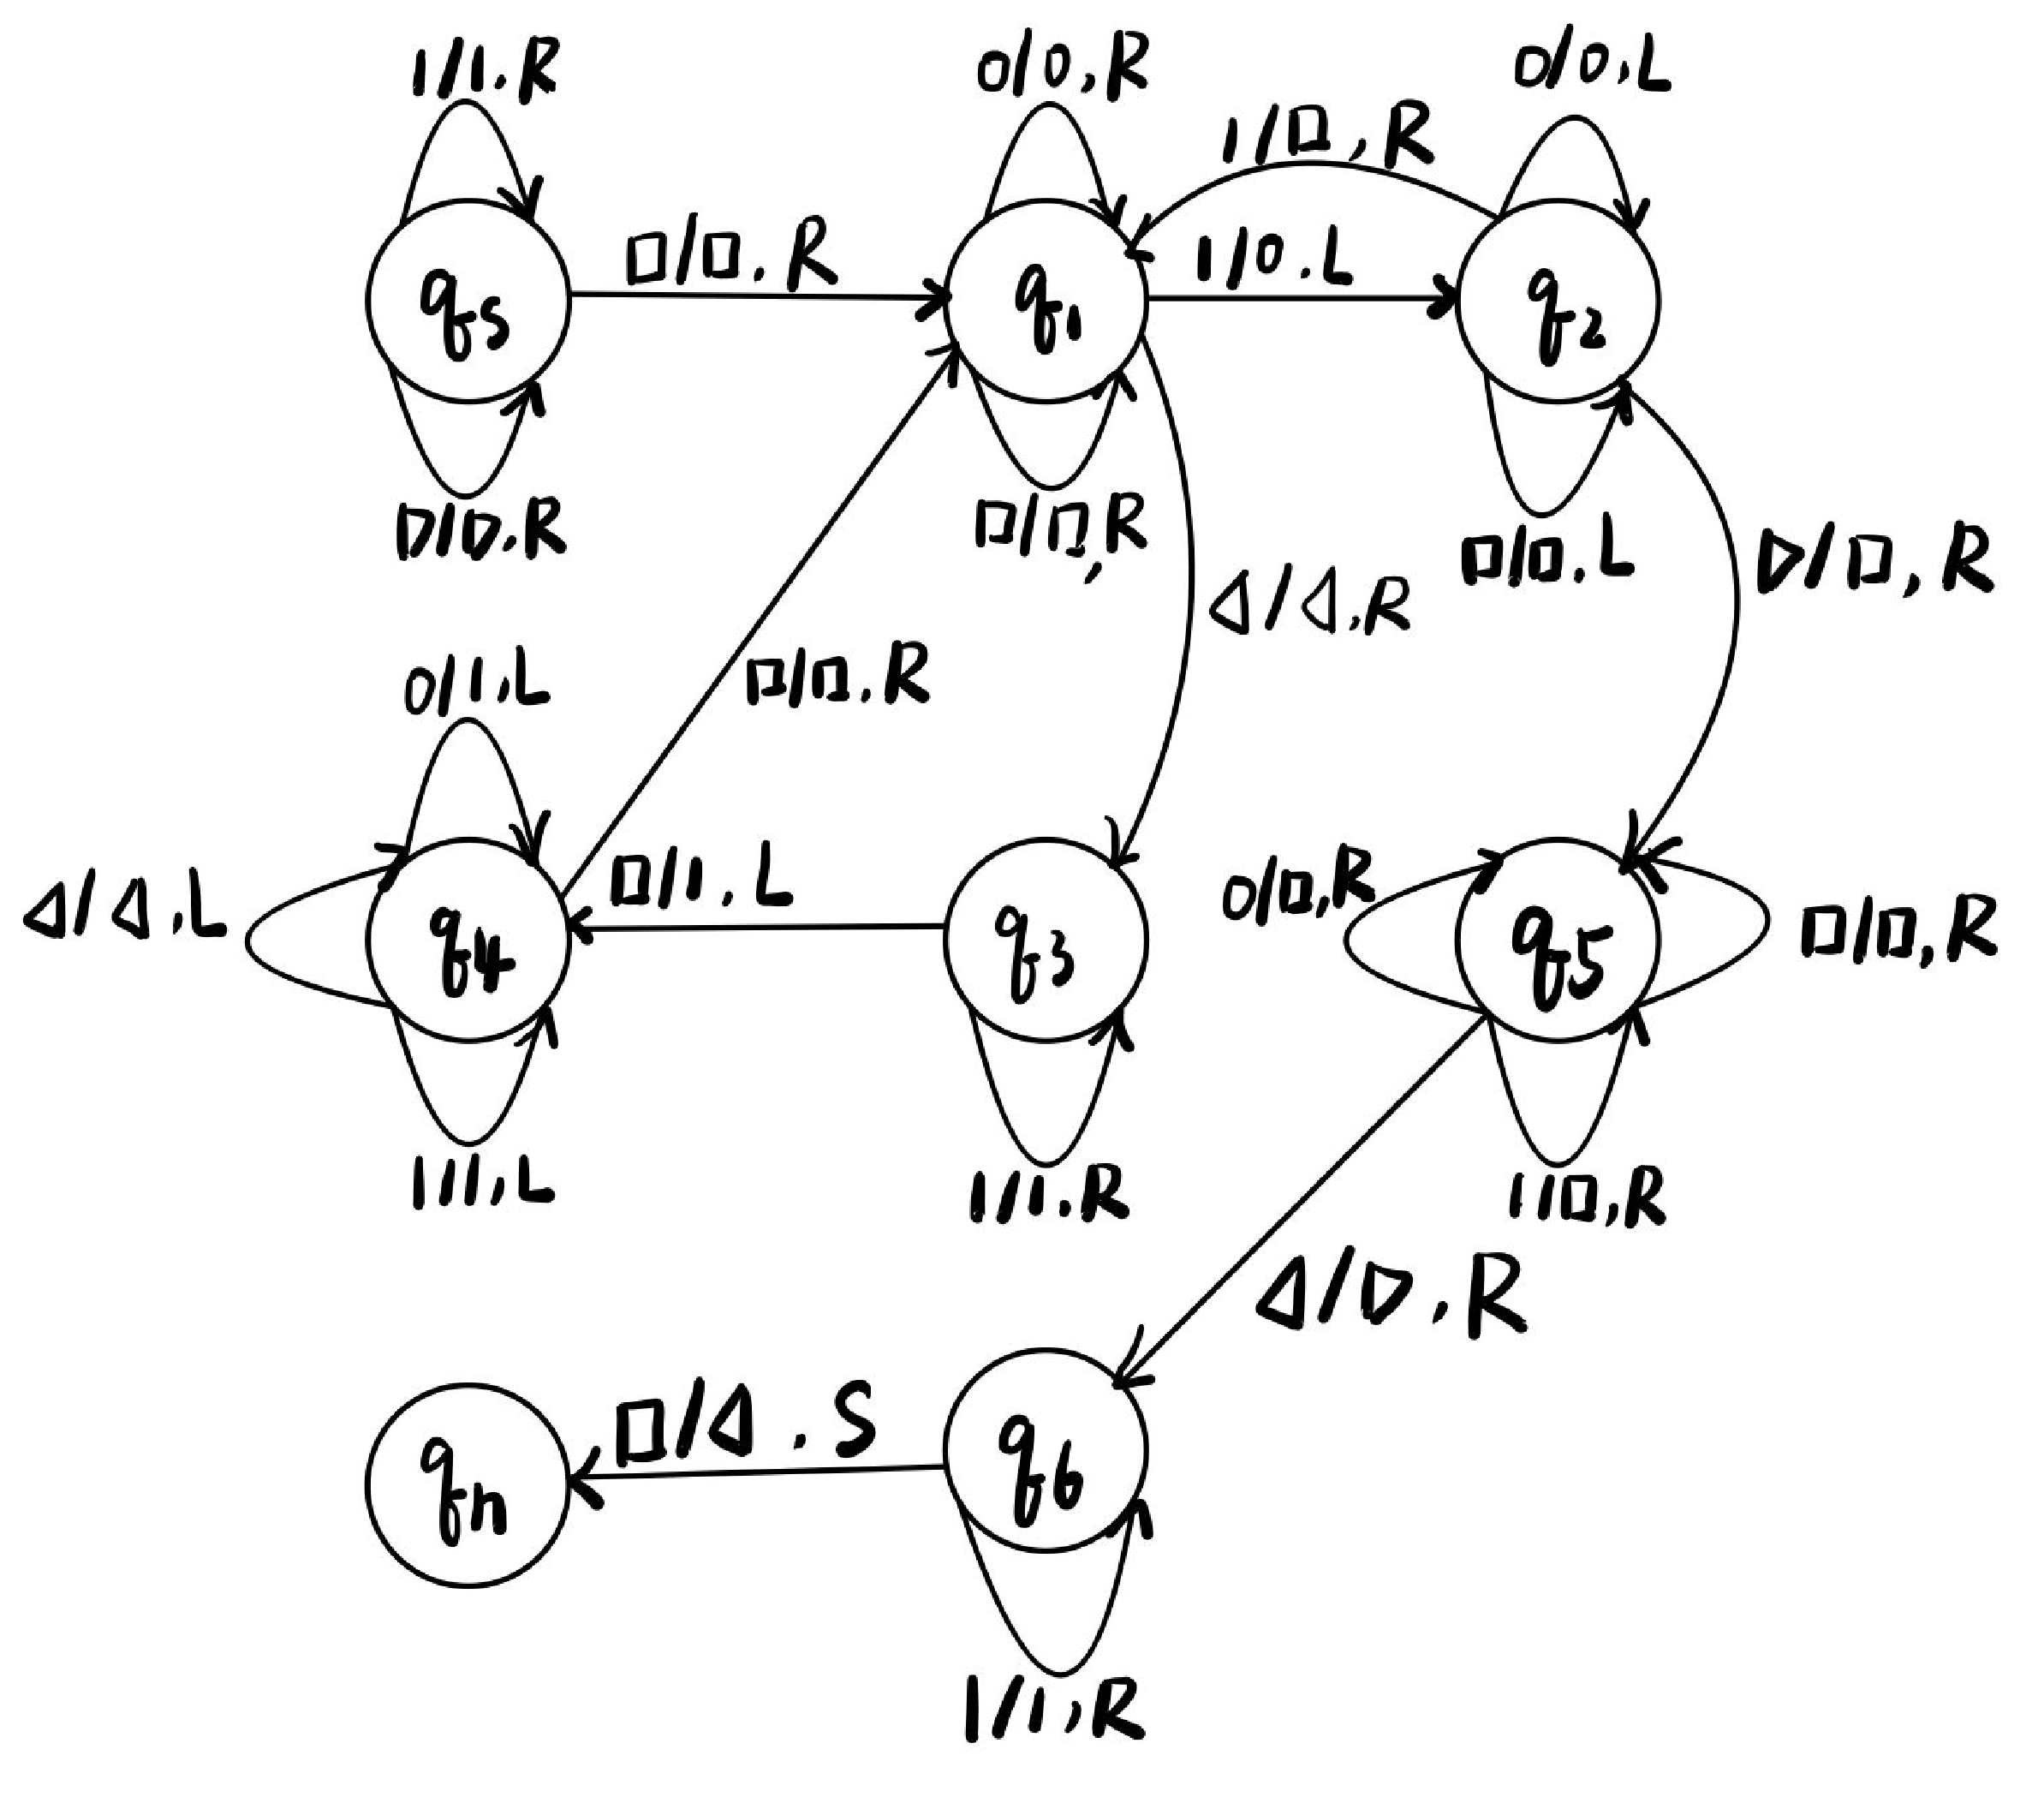
\includegraphics[width=0.8\textwidth]{Fig-Graph.pdf}
	\caption{State transition diagram.}
	\label{Fig-diagram}
	\end{figure}
	\item \textbf{\textit{The whole process:}}
	\begin{align*}\nonumber
		&(q_s,\underline{\triangleright}1111111\Box 111\triangleleft)\vdash^* (q_s,\triangleright 1111111\underline{\Box} 111\triangleleft)
\vdash  (q_1,\triangleright 1111111\Box\underline{1} 11\triangleleft)\\
\vdash &(q_2,\triangleright 1111111\underline{\Box} 011\triangleleft)
\vdash 	(q_2,\triangleright 111111\underline{1}\Box 011\triangleleft)
\vdash  (q_1,\triangleright 111111\Box\underline{\Box} 011\triangleleft)\\
\vdash &(q_1,\triangleright 111111\Box\Box\underline{0} 11\triangleleft)
\vdash  (q_1,\triangleright 111111\Box\Box 0 \underline{1} 1\triangleleft)
\vdash^* (q_2,\triangleright 111111\Box\underline{\Box}00 1\triangleleft)\\
\vdash^* &(q_2,\triangleright 11111\underline{1}\Box\Box 00 1\triangleleft)
\vdash (q_1,\triangleright 11111\Box\underline{\Box}\Box 00 1\triangleleft)
\vdash^* (q_1,\triangleright 11111\Box\Box\Box \underline{0}0 1\triangleleft)\\
\vdash^*&(q_1,\triangleright 11111\Box\Box\Box 00 \underline{1}\triangleleft)
\vdash (q_2,\triangleright 11111\Box\Box\Box 0 \underline{0} 0\triangleleft)
\vdash^* (q_2,\triangleright 11111\Box\Box\underline{\Box} 000\triangleleft)\\
\vdash^*&(q_2,\triangleright 1111\underline{1}\Box\Box\Box 000\triangleleft)
\vdash (q_1,\triangleright 1111\Box\underline{\Box}\Box\Box 000\triangleleft)
\vdash^*(q_1,\triangleright 1111\Box\Box\Box\Box\underline{0}00\triangleleft)\\
\vdash^*&(q_1,\triangleright 1111\Box\Box\Box\Box000\underline{\triangleleft})
\vdash (q_3,\triangleright 1111\Box\Box\Box\Box000\triangleleft\underline{\Box})
\vdash (q_4,\triangleright 1111\Box\Box\Box\Box000\underline{\triangleleft} 1)\\
\vdash&(q_4,\triangleright 1111\Box\Box\Box\Box00\underline{0}\triangleleft 1)
\vdash*(q_4,\triangleright 1111\Box\Box\Box\underline{\Box}111\triangleleft 1)
\vdash(q_1,\triangleright 1111\Box\Box\Box\Box\underline{1}11\triangleleft 1)\\
\vdash&(q_2,\triangleright 1111\Box\Box\Box\underline{\Box}011\triangleleft 1)
\vdash^*(q_2,\triangleright 111\underline{1}\Box\Box\Box\Box 011\triangleleft 1)
\vdash (q_1,\triangleright 111\Box\underline{\Box}\Box\Box\Box 011\triangleleft 1)\\
\vdash*&(q_1,\triangleright 111\Box\Box\Box\Box\Box \underline{0}11\triangleleft 1)
\vdash (q_1,\triangleright 111\Box\Box\Box\Box\Box 0 \underline{1}1\triangleleft 1)
\vdash (q_2,\triangleright 111\Box\Box\Box\Box\Box  \underline{0}01\triangleleft 1)\\
\vdash&(q_2,\triangleright 111\Box\Box\Box\Box\underline{\Box} 001\triangleleft 1)
\vdash^* (q_2,\triangleright 11\underline{1}\Box\Box\Box\Box\Box 001\triangleleft 1)
\vdash (q_1,\triangleright 11\Box\underline{\Box}\Box\Box\Box\Box 001\triangleleft 1)\\
\vdash^*&(q_1,\triangleright 11\Box\Box\Box\Box\Box\Box \underline{0}01\triangleleft 1)
\vdash^* (q_1,\triangleright 11\Box\Box\Box\Box\Box\Box 00\underline{1}\triangleleft 1)
\vdash (q_2,\triangleright 11\Box\Box\Box\Box\Box\Box 0\underline{0}0\triangleleft 1)\\
\vdash^*&(q_2,\triangleright 11\Box\Box\Box\Box\Box\underline{\Box} 000\triangleleft 1)
\vdash^* (q_2,\triangleright 1\underline{1}\Box\Box\Box\Box\Box\Box 000\triangleleft 1)
\vdash (q_1,\triangleright 1\Box\underline{\Box}\Box\Box\Box\Box\Box 000\triangleleft 1)\\
\vdash^*&(q_1,\triangleright 1\Box\Box\Box\Box\Box\Box\Box \underline{0}00\triangleleft 1)
\vdash^* (q_1,\triangleright 1\Box\Box\Box\Box\Box\Box\Box 000\underline{\triangleleft} 1)
\vdash (q_3,\triangleright 1\Box\Box\Box\Box\Box\Box\Box 000\triangleleft \underline{1})\\
\vdash&(q_3,\triangleright 1\Box\Box\Box\Box\Box\Box\Box 000\triangleleft 1 \underline{\Box})
\vdash (q_4,\triangleright 1\Box\Box\Box\Box\Box\Box\Box 000\triangleleft \underline{1} 1)
\vdash (q_4,\triangleright 1\Box\Box\Box\Box\Box\Box\Box 000\underline{\triangleleft} 1 1)\\
\vdash&(q_4,\triangleright 1\Box\Box\Box\Box\Box\Box\Box 00\underline{0}\triangleleft 1 1)
\vdash^*(q_4,\triangleright 1\Box\Box\Box\Box\Box\Box\underline{\Box} 111\triangleleft 1 1)
\vdash(q_1,\triangleright 1\Box\Box\Box\Box\Box\Box\Box \underline{1} 11\triangleleft 1 1)\\
\vdash&(q_2,\triangleright 1\Box\Box\Box\Box\Box\Box\underline{\Box} 0 11\triangleleft 1 1)
\vdash^*(q_2,\triangleright \underline{1}\Box\Box\Box\Box\Box\Box\Box 0 11\triangleleft 1 1)
\vdash (q_1,\triangleright \Box\underline{\Box}\Box\Box\Box\Box\Box\Box 0 11\triangleleft 1 1)\\
\vdash^*& (q_1,\triangleright \Box\Box\Box\Box\Box\Box\Box\Box 0 \underline{1}1\triangleleft 1 1)
\vdash (q_2,\triangleright \Box\Box\Box\Box\Box\Box\Box\Box \underline{0} 01\triangleleft 1 1)
\vdash^*(q_2,\underline{\triangleright} \Box\Box\Box\Box\Box\Box\Box\Box 001\triangleleft 1 1)\\
\vdash&(q_5,\Box \underline{\Box}\Box\Box\Box\Box\Box\Box\Box 001\triangleleft 1 1)
\vdash^*(q_6,\Box\Box\Box\Box\Box\Box\Box\Box\Box \Box\Box\Box\triangleright
 \underline{1} 1)\\
 \vdash^*&(q_6,\Box\Box\Box\Box\Box\Box\Box\Box\Box \Box\Box\Box\triangleright
 1 1\underline{\Box})\\
 \vdash &(q_{halt},\Box\Box\Box\Box\Box\Box\Box\Box\Box \Box\Box\Box\triangleright
 1 1\underline{\triangleleft})
	\end{align*}
	\end{enumerate}
	\end{solution}	
	
	
    \item 
    Given the alphabet $\{1, 0, \Box, \triangleright, \triangleleft\}$, design a time efficient 3-tape TM $M$ to compute $f:\{0,1\}^*\rightarrow\{0,1\}$ which verifies whether the number of 0 and the number of 1 are the same in an input consisting of only 0's and 1's. $M$ should output 1 if the numbers are the same, and 0 otherwise. For eample, for the input tape $\triangleright 001101\triangleleft$, $M$ should output 1
    
    \begin{enumerate}
	    \item
	    Please describe your design and then write the specifications of $M$ in the form like $\langle q_S, \triangleright, \triangleright, \triangleright \rangle \rightarrow \langle q_1, \triangleright,\triangleright,  R, R, S \rangle$. Explain the transition functions in detail.
	    
	    \item 
	    Show the time complexity for one-tape TM $M'$ to compute the same function $f$ with $n$ symbols in the input and give a brief description of such $M'$ .
	
	\end{enumerate}
	\begin{solution}
	~\\
	\begin{enumerate}
	\item \textbf{\textit{Transition functions:}}
	\begin{align*}\nonumber
	Start\ state\\
	&<q_s,\triangleright,\triangleright,\triangleright>\rightarrow <q_c,\triangleright,\triangleright,R,R,R>\\
	~\\
	Begin\ to\ copy\\
	&<q_c,1,\Box,\Box>\rightarrow <q_c,1,\Box,R,R,S>\\
	&<q_c,0,\Box,\Box>\rightarrow <q_c,\Box,\Box,R,S,S>\\
	&<q_c,\triangleleft,\Box,\Box>\rightarrow <q_t,\Box,\Box,L,L,S>\\	
	~\\	
	Begin\ to\ compare\\
	&<q_t,0,1,\Box>\rightarrow <q_t,1,\Box,L,L,S>\\
	&<q_t,1,1,\Box>\rightarrow <q_t,1,\Box,L,S,S>\\
	&<q_t,0,\triangleright,\Box>\rightarrow <q_r,\triangleright,0,S,S,R>\\
	&<q_t,\triangleright,\triangleright,\Box>\rightarrow <q_r,\triangleright,1,S,S,R>\\
	&<q_t,1,\triangleright,\Box>\rightarrow <q_r,\triangleright,\Box,L,S,S>\\
	~\\
	Ready\ to\ terminate\\
	&<q_r,0,\triangleright,\Box>\rightarrow <q_h,\triangleright,\triangleleft,S,S,S>\\
	&<q_r,\triangleright,\triangleright,\Box>\rightarrow <q_h,\triangleright,\triangleleft,S,S,S>\\
	\end{align*}
	\textbf{\textit{Explanation:}}
	\\
	\textbf{State $q_s$} is the starting state where the three heads are reading $\triangleright$. Move them right without writing to starting executing the Turing Machine.
	\\
	\textbf{State $q_c$} copies all the $1$s in the input sequence to the second tape.
	\\
	\textbf{State $q_t$} compares the contents of the first tape with that of the second tape. Since the second head always reads $1$ before reading $\triangleright$, if the first head reads $0$, both of them will move to the next position; else if the first head reads $1$, the first head will move to the next position while the second one will stay. After many times of such operation, the loop will terminate with reading $<\triangleright,\triangleright>$ or $<0,\triangleright>$. The situation of $<0,\triangleright>$ the number of $0$s is bigger than that of $1$s while the other situation mean the number of $0$s is equal to that of $1$S.
	\\
	\textbf{State $q_r$} formats the output by adding $\triangleleft$ to the end of result and transform the state to $h_{halt}$ to stop executing. 
	
	\item 
	\textbf{\textit{Time complexity of M':}} Assume that the initial problem is computable in time $T(n)$ by a Turing Machine $M$ with three tapes, then it is computable in time $15T(n)^2$ by a single-tape Turing machine $\tilde{M}$.
	\\
	\textbf{\textit{Brief description:}} The machine $\tilde{M}$ places $\triangleright$ after the input sequence and then start copying the input to the imaginary input tape.During this process whenever an input symbol is copied it is overwritten by $\triangleright$.
	\\
	The $n+2$-cell and $n+3$-cell indicate the initial head position while the $n+1$-cell is reserved for the input. $\tilde{M}$ sweeps $kT(n)$ cells from the $n+1$-cell the right and $kT(n)$ cell form right to left to update using the transitions of $M$.
	\end{enumerate}
	\end{solution}
	\item Define the corresponding decision or search problem of the following problems and give the "certificate" and "certifier" for each decision problem provided in the subquestions or defined by yourself.
	
	\begin{enumerate}
	    \item
	    \textit{3-Dimensional Matching.}  Given disjoint sets $X,Y,Z$ all with the size of $n$, and a set $M \subseteq X\times Y\times Z$.  Is there a subset $M'$ of $M$ of size $n$ where no two elements of $M'$ agree in any coordinate?
	    
	    \item 
	    \textit{Travelling Salesman Problem.} Given a list of cities and the distances between each pair of cities, find the shortest possible route that visits each city exactly once and returns to the origin city.
	    
	    \item
	    \textit{Job Sequencing.} Given a set of unit-time jobs, each of which has an integer deadline and a nonnegative penalty for missing the deadline. Does there exist a job sequence that has a total penalty $w\leqslant k$?
	    
	\end{enumerate}
	\begin{solution}
	~\\
	\begin{enumerate}
	\item 
	It is a \textbf{decision problem}, the corresponding search problem is: \textit{Given disjoint sets $X$,$Y$, and $Z$, find a subset $M'$ of $M$ of size $n$ where no two elements of $M'$ agree in any coordinate}.
	\\
	\textbf{\textit{Certificate:}} A pair of triplets $t$ in $M'$ with at least one of their coordinates agree. Note that such a certificate exists iff the set $M'$ doesn't exist.
	\\
	\textbf{\textit{Certifier:}} Check each pair of triplets of possible $M'$ to determine whether such a set exists or not.
	\item
	It is a \textbf{search problem}, the corresponding decision problem is: \textit{Is there a possible route with total distance less than $k$, which visits each city exactly once and returns to the origin city.}
	\\
	\textbf{\textit{Certificate:}} All the possible travelling routines.
	\\
	\textbf{\textit{Certifier:}} If there exists a path satisfying that it visits each city once and returns to the origin city, check if the total distance is less than k. If the proposition is true, the decision problem is true. Vice versa.
	\item
	It is a \textbf{decision problem}, the corresponding search problem is: \textit{Given such unit-time jobs, find the job sequence with the least total penalty}.
	\\
	\textbf{\textit{Certificate:}} All the possible job sequences.
	\\
	\textbf{\textit{Certifier:}} Check each possible job sequence and compute the total penalty, if the total penalty is less or equal than $k$, the original proposition is true.
	\end{enumerate}
	\end{solution}
\end{enumerate}

\textbf{Remark:} Please include your .pdf, .tex files for uploading with standard file names.
\newpage


%========================================================================
\end{document}